\documentclass[12pt]{article}
\usepackage{fullpage,amsmath,amssymb,amsfonts,amsthm}
\usepackage[utf8]{inputenc}
\usepackage[english]{babel}
\usepackage{graphics}
\usepackage{tikz}
\usepackage{pgfplots}

\pgfplotsset{compat=1.8}
\title{Performance Report}

\begin{document}

\maketitle

\begin{figure}[h!]
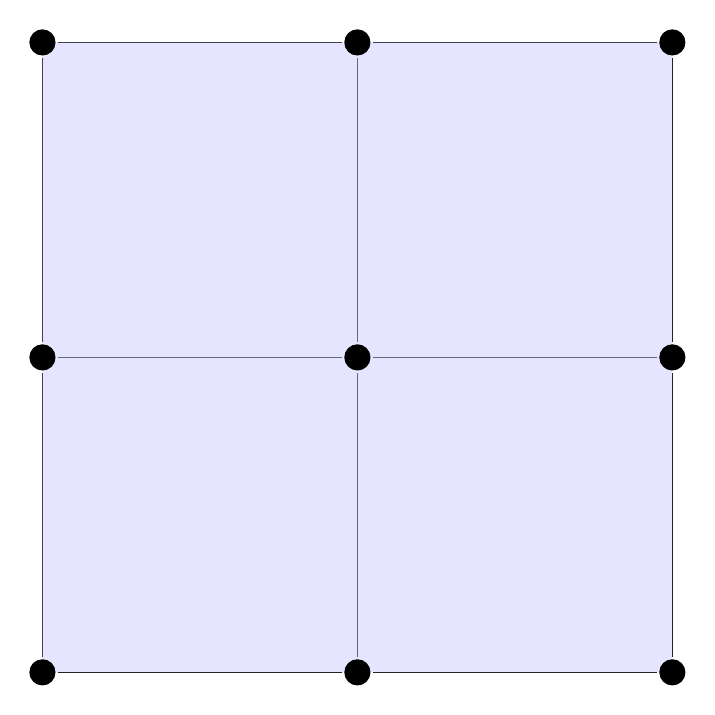
\begin{tikzpicture}[scale=4.00, every node/.style={scale=1.60}]

%vertex labels
\draw
	(0.000000,0.000000) node (v0) {}
	(1.000000,0.000000) node (v1) {}
	(0.000000,1.000000) node (v2) {}
	(1.000000,1.000000) node (v3) {}
	(2.000000,0.000000) node (v4) {}
	(2.000000,1.000000) node (v5) {}
	(0.000000,2.000000) node (v6) {}
	(1.000000,2.000000) node (v7) {}
	(2.000000,2.000000) node (v8) {};

%plot non-open edges
\draw
	(v0)--(v1)
	(v1)--(v3)
	(v3)--(v2)
	(v2)--(v0)
	(v1)--(v4)
	(v4)--(v5)
	(v5)--(v3)
	(v3)--(v7)
	(v7)--(v6)
	(v6)--(v2)
	(v5)--(v8)
	(v8)--(v7);

%plot open edges
\draw[very thick, dashed];

%fill faces
\fill[color=blue!20, opacity=.5] 
	(v0.center)--(v1.center)--(v3.center)--(v2.center)--cycle
	(v1.center)--(v4.center)--(v5.center)--(v3.center)--cycle
	(v3.center)--(v2.center)--(v6.center)--(v7.center)--cycle
	(v5.center)--(v3.center)--(v7.center)--(v8.center)--cycle;

%plot non-open vertices
\draw
	(v0) node[draw, circle, inner sep=2pt, fill=black] {}
	(v1) node[draw, circle, inner sep=2pt, fill=black] {}
	(v2) node[draw, circle, inner sep=2pt, fill=black] {}
	(v3) node[draw, circle, inner sep=2pt, fill=black] {}
	(v4) node[draw, circle, inner sep=2pt, fill=black] {}
	(v5) node[draw, circle, inner sep=2pt, fill=black] {}
	(v6) node[draw, circle, inner sep=2pt, fill=black] {}
	(v7) node[draw, circle, inner sep=2pt, fill=black] {}
	(v8) node[draw, circle, inner sep=2pt, fill=black] {};

%plot open vertices
\draw;

\end{tikzpicture}
\hspace{.2cm}
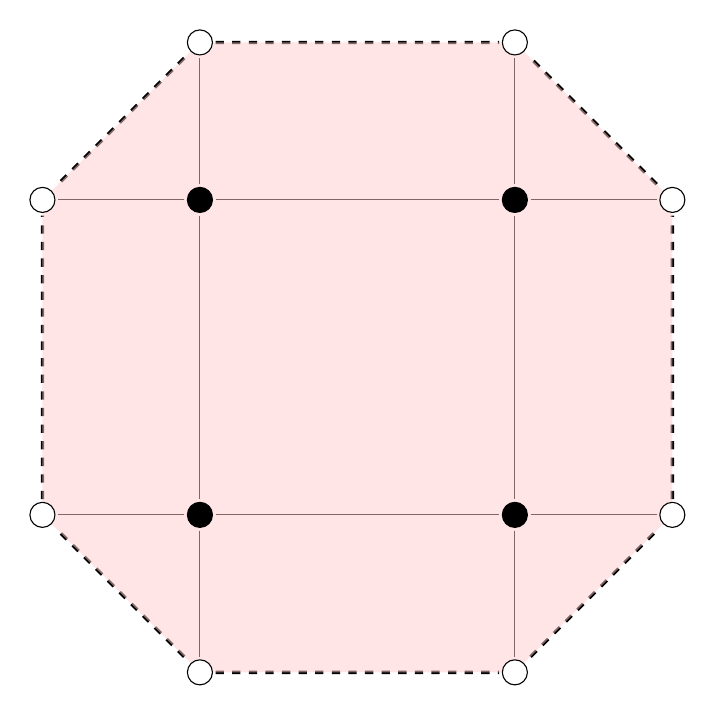
\begin{tikzpicture}[scale=4.00, every node/.style={scale=1.60}]

%vertex labels
\draw
	(0.500000,0.500000) node (v0) {}
	(1.500000,0.500000) node (v1) {}
	(0.500000,1.500000) node (v2) {}
	(1.500000,1.500000) node (v3) {}
	(0.500000,0.000000) node (v4) {}
	(0.000000,0.500000) node (v5) {}
	(1.500000,0.000000) node (v6) {}
	(2.000000,0.500000) node (v7) {}
	(0.500000,2.000000) node (v8) {}
	(0.000000,1.500000) node (v9) {}
	(2.000000,1.500000) node (v10) {}
	(1.500000,2.000000) node (v11) {};

%plot non-open edges
\draw
	(v0)--(v4)
	(v0)--(v1)
	(v0)--(v2)
	(v0)--(v5)
	(v1)--(v6)
	(v1)--(v7)
	(v1)--(v3)
	(v2)--(v3)
	(v2)--(v8)
	(v2)--(v9)
	(v3)--(v10)
	(v3)--(v11);

%plot open edges
\draw[very thick, dashed]
	(v4)--(v5)
	(v4)--(v6)
	(v5)--(v9)
	(v6)--(v7)
	(v7)--(v10)
	(v8)--(v9)
	(v8)--(v11)
	(v10)--(v11);

%fill faces
\fill[color=red!20, opacity=.5] 
	(v0.center)--(v4.center)--(v5.center)--cycle
	(v0.center)--(v4.center)--(v6.center)--(v1.center)--cycle
	(v0.center)--(v2.center)--(v9.center)--(v5.center)--cycle
	(v0.center)--(v1.center)--(v3.center)--(v2.center)--cycle
	(v1.center)--(v6.center)--(v7.center)--cycle
	(v1.center)--(v7.center)--(v10.center)--(v3.center)--cycle
	(v2.center)--(v8.center)--(v9.center)--cycle
	(v2.center)--(v3.center)--(v11.center)--(v8.center)--cycle
	(v3.center)--(v10.center)--(v11.center)--cycle;

%plot non-open vertices
\draw
	(v0) node[draw, circle, inner sep=2pt, fill=black] {}
	(v1) node[draw, circle, inner sep=2pt, fill=black] {}
	(v2) node[draw, circle, inner sep=2pt, fill=black] {}
	(v3) node[draw, circle, inner sep=2pt, fill=black] {};

%plot open vertices
\draw
	(v4) node[draw, circle, inner sep=2pt, fill=white] {}
	(v5) node[draw, circle, inner sep=2pt, fill=white] {}
	(v6) node[draw, circle, inner sep=2pt, fill=white] {}
	(v7) node[draw, circle, inner sep=2pt, fill=white] {}
	(v8) node[draw, circle, inner sep=2pt, fill=white] {}
	(v9) node[draw, circle, inner sep=2pt, fill=white] {}
	(v10) node[draw, circle, inner sep=2pt, fill=white] {}
	(v11) node[draw, circle, inner sep=2pt, fill=white] {};

\end{tikzpicture}
\caption{The tiling and its dual tiling}
\end{figure}
\vspace{.2cm}

\newpage
\begin{table}[h]
\centering
\begin{tabular}{c c}
\hline
Number of physical qubits & $n = 12$ \\
\hline
Number of logical qubits & $k = 0$\\
\hline
Overhead & $n/k = inf$\\
\hline
\end{tabular}
\caption{Error-correction overhead}
\end{table}
\vspace{.3cm}


\begin{table}[h]
\centering
\begin{tabular}{c c}
\hline
weight & number of $Z$-measurements\\
\hline
4 & 4\\
\hline
\hline
weight & number of $X$-measurements\\
\hline
2 & 4\\
3 & 4\\
4 & 1\\
\hline
\end{tabular}
\caption{Measurements weight distribution}
\end{table}
\vspace{.3cm}



\vspace{2cm}
Total simulation time: $< 1$ second.
\end{document}